\documentclass[12pt]{article}

\usepackage[utf8]{inputenc}
\usepackage[margin=1in]{geometry}
\renewcommand{\baselinestretch}{1}
\usepackage{indentfirst}

\usepackage{amsmath, amssymb}

\usepackage{hyperref}
\usepackage{cleveref}
\usepackage{graphicx}
\usepackage{float}
\graphicspath{{./figs/}}

\usepackage{natbib}
\bibliographystyle{aasjournal}

\begin{document}

\begin{center}\begin{LARGE}
\textbf{ASTR 5463: Accelerated Lambda Iteration}
\end{LARGE}\end{center}

\begin{center}
\textbf{Manuel Barrientos, Anthony Burrow, Adam Moss, Sarah Stangl}
\end{center}


\section{Introduction}


One of the most fundamental problems in stellar atmospheres is being able to solve two equations simultaneously, the radiative transfer equation and the statistical equilibrium equation \citep[e.g.,][]{OandK1987,hubeny2003}. The first one is given for the plane-parallel case as
\begin{align}
\mu \frac{d I_\nu(\mu, \tau)}{d \tau_\nu}
&=
I_\nu(\mu, \tau_\nu) - S_\nu(\tau_\nu),
\end{align}
where $I_\nu(\mu, \tau_\nu)$ is the specific intensity and $S_\nu$ the source function. The former depends on the directional cosine $\mu$, the monochromatic optical depth $\tau_\nu$, and both quantities depend on the frequency $\nu$. Because of the complicated coupling of the quantities in this equation, the formal solution to this integral-differential equation must be solved numerically. The first-moment equation may be written as
\begin{align}
J_\nu
&=
\Lambda_\nu S_\nu,
\label{eq:2}
\end{align}
with $\Lambda_\nu$ being a wavelength-dependent operator that may act on $S(\tau)$, and
\begin{align}
J_\nu(\tau)
&=
\frac{1}{2} \int_{-1}^1 I_\nu(\mu, \tau_\nu) d\mu
\end{align}
is the mean intensity. The second one can be expressed as the source function
\begin{align}
S_\nu
&=
(1 - \epsilon) J_\nu + \epsilon B_\nu,
\label{eq:4}
\end{align}
where $\epsilon$ is the thermalization (also known as the collisional destruction probability), and $B_\nu$ is the Planck function. Combining Equations \ref{eq:2} and \ref{eq:4}, this may be written as
\begin{align}
S_\nu
&=
(1 - \epsilon) \Lambda_\nu S_\nu + \epsilon B_\nu,
\end{align}
or in other words,
\begin{align}
S_\nu
&=
[1 - (1 - \epsilon) \Lambda_\nu]^{-1} \epsilon B_\nu,
\end{align}
However, because this equation must be solved numerically, and $\Lambda_\nu$ is typically expressible as an $N \times N$ matrix, where $N$ is the number of points on the $\tau$ grid used, inverting this matrix quickly becomes computationally expensive. It is therefore important to explore faster and more efficient methods of solving the formal solution.

The formal solution can instead be solved using an iterative method by converging $J_\nu$. By iteratively applying the lambda operator to the source function $S_\nu$, the approximation for $J_\nu$ is improved with each iteration. This lambda iteration may be written as
\begin{align}
S^{(n + 1)}_\nu
&=
(1 - \epsilon) \Lambda_\nu S^{(n)}_\nu + \epsilon B_\nu.
\end{align}
for some $n^\text{th}$ iteration of calculating $S_\nu$ from $J_\nu$. This approach avoids the need to invert $\Lambda_\nu$. However, for cases of highly non-local thermal equilibrium (non-LTE or NLTE) where $\epsilon \ll 1$, the convergence time is slow \citep[see, e.g.,][]{mihalas1978}. In this case, the relative changes in the source function become extremely small long before the correct solution is reached \citep[see][]{hubeny2003}.

Because of this, a more efficient technique for solving this equation is needed. In particular, accelerated lambda iteration (ALI) has been put into context of the short-characteristics method (see \autoref{sec:numerical_approach}) by \cite{OandK1987}, which will henceforth be referred to as O\&K. As explained by O\&K, one may consider introducing a perturbation operator $\Lambda^*_\nu$ that contains information about the dominant physics of line-core diffusion. We can then define the exact lambda operator as
\begin{align}
\Lambda_\nu
&=
\Lambda^*_\nu + (\Lambda_\nu - \Lambda^*_\nu).
\end{align}
From here one may create a new iteration method by attributing the first term in this lambda operator to the $(n + 1)^\text{th}$ iteration, and the other terms to the previous $n^\text{th}$ iteration; in other words,
\begin{align}
S^{(n + 1)}_\nu
&=
(1 - \epsilon) \Lambda^*_\nu S^{(n + 1)}_\nu + (1 - \epsilon) (\Lambda_\nu - \Lambda^*_\nu) S^{(n)}_\nu + \epsilon B_\nu,
\end{align}
which becomes
\begin{align}
[1 - (1 - \epsilon) \Lambda^*_\nu] S^{(n + 1)}_\nu
&=
(1 - \epsilon) (\Lambda_\nu - \Lambda^*_\nu) S^{(n)}_\nu + \epsilon B_\nu.
\end{align}
One may also write this in terms of $J_\nu$ as
\begin{align}
J_\nu^{(n + 1)} - J_\nu^{(n)}
&=
[1 - (1 - \epsilon) \Lambda^*_\nu]^{-1} (J_\nu^{FS, (n)} - J_\nu^{(n)})
\label{eq:11}
\end{align}
where $J^{FS, (n)} = \Lambda_\nu S^{(n)}$. This may then be used with equation \ref{eq:4} to complete a full ALI cycle.

The advantage of this new iteration scheme is that, when an appropriate perturbation $\Lambda^*_\nu$ is chosen, such as a diagonal or multi-banded diagonal matrix, we may perform the matrix inversion quickly, with $\mathcal{O}(n)$ time, rather than near $\mathcal{O}(n^3)$ time for typical matrix inversion. At the same time, the convergence procedure is accelerated because introducing the perturbation matrix reduces the eigenvalues of the lambda matrix. Typically this perturbation matrix is chosen to be the diagonals, tri-diagonals, or higher-order banded diagonals of the lambda operator.

In this project, we aim to solve the radiative transfer equation and simultaneously scattering problem for a generally NLTE plane-parallel atmosphere. We specifically perform ALI to do so, and we also add further optimizations to this method, which are described in \autoref{sec:methods} along with assumptions we make to conquer this problem. In \autoref{sec:results}, results of our work are shown, and we discuss what these results suggest.


\section{Methods}
\label{sec:methods}


\subsection{Numerical Approach}
\label{sec:numerical_approach}


To perform ALI, we first use the short-characteristics method of solving the formal solution given by O\&K. This method solves the set of equations
\begin{align}
\begin{split}
I^+_\nu(\tau_\nu, \mu)
&=
I^+_\nu(T_\nu, \mu) e^{-(T_\nu - \tau_\nu) / \mu} + \int_{\tau_\nu}^{T_\nu} S_\nu(t) e^{-(t - \tau_\nu) / \mu} dt / \mu,
\\
I^-_\nu(\tau_\nu, \mu)
&=
I^+_\nu(0, \mu) e^{\tau_\nu / \mu} + \int_0^{\tau_\nu} S_\nu(t) e^{-(\tau_\nu - t) / \mu} dt / (-\mu),
\end{split}
\end{align}
where $I^+_\nu$ and $I^-_\nu$ are outward-going and inward-going rays, respectively, and $T_\nu$ is the monochromatic slab thickness. To solve this, the short-characteristics method performs integration by interpolating $S_\nu(\tau)$ at each set of two to three adjacent points. This can be written as
\begin{align}
\begin{split}
I^+(\tau_i, \mu)
&=
I^+(\tau_{i + 1}, \mu) e^{-\Delta\tau_i} + \Delta I^+(S, \mu),
\\
I^-(\tau_i, \mu)
&=
I^-(\tau_{i - 1}, \mu) e^{-\Delta\tau_{i - 1}} + \Delta I^-(S, \mu),
\label{eq:13}
\end{split}
\end{align}
where $\Delta I^\pm$ represents the integral evaluations, and $\Delta \tau_i = (\tau_{i + 1} - \tau_i) / |\mu|$. We also have left out the $\nu$ subscripts for convenience; note that this process must still be performed for each wavelength point on the chosen grid. This can be written in terms of interpolation coefficients $\alpha^\pm_i$, $\beta^\pm_i$, $\gamma^\pm_i$ as
\begin{align}
\Delta I^\pm_i
&=
\alpha^\pm_i S_{i - 1} + \beta^\pm_i S_i + \gamma^\pm_i S_{i + 1}.
\label{eq:16}
\end{align}
O\&K gives parabolic interpolation coefficients as
\begin{align}
\begin{split}
\alpha_i^-
&=
e_{0, i} +
\frac{e_{2, i} - (\Delta\tau_i + 2\Delta\tau_{i - 1}) e_{1, i}}
     {\Delta\tau_{i - 1} (\Delta\tau_i + \Delta\tau_{i - 1})},
\\
\beta_i^-
&=
\frac{(\Delta\tau_i + \Delta\tau_{i - 1}) e_{1, i} - e_{2, i}}
     {\Delta\tau_{i - 1} \Delta\tau_i},
\\
\gamma_i^-
&=
\frac{e_{2, i} - \Delta\tau_{i - 1} e_{1, i}}
     {\Delta\tau_i (\Delta\tau_i + \Delta\tau_{i - 1})},
\\
\alpha_i^+
&=
\frac{e_{2, i + 1} - \Delta\tau_i e_{1, i + 1}}
     {\Delta\tau_{i - 1} (\Delta\tau_i + \Delta\tau_{i - 1})},
\\
\beta_i^+
&=
\frac{(\Delta\tau_i + \Delta\tau_{i - 1}) e_{1, i + 1} - e_{2, i + 1}}
     {\Delta\tau_{i - 1} \Delta\tau_i},
\\
\gamma_i^+
&=
e_{0, i + 1} +
\frac{e_{2, i + 1} - (\Delta\tau_{i - 1} + 2\Delta\tau_i) e_{1, i + 1}}
     {\Delta\tau_i (\Delta\tau_i + \Delta\tau_{i - 1})},
\end{split}
\end{align}
where
\begin{align}
\begin{split}
e_{0, i}
&=
1 - e^{-\Delta\tau_{i - 1}},
\\
e_{1, i}
&=
\Delta\tau_{i - 1} - e_{0, i}
\\
e_{2, i}
&=
(\Delta\tau_{i - 1})^2 - 2 e_{1, i}.
\end{split}
\end{align}
For the boundaries $i = 1$ and $i = N$, linear interpolation must be performed instead; O\&K gives the linear interpolation coefficients as
\begin{align}
\begin{split}
\alpha_i^-
&=
e_{0, i} - \frac{e_{1, i}}{\Delta \tau_{i - 1}},
\\
\beta_i^-
&=
\frac{e_{1, i}}{\Delta \tau_{i - 1}},
\\
\gamma_i^-
&=
0,
\\
\alpha_i^+
&=
0,
\\
\beta_i^+
&=
\frac{e_{1, i + 1}}{\Delta \tau_i},
\\
\gamma_i^+
&=
e_{0, i + 1} - \frac{e_{1, i + 1}}{\Delta \tau_i}.
\end{split}
\end{align}
At low $\Delta \tau_i < 10^{-2}$, we also enforce the use of linear interpolation as well to avoid numerical problems. It should also be noted that, to also avoid problems with exponentials at very low $\Delta \tau_i < 10^{-7}$, the $e^{-\Delta \tau_i}$ have have been Taylor-expanded to second order, and $e_{0, i}$, $e_{1, i}$, and $e_{2, i}$ were adjusted accordingly to appropriately estimate our results when we want to resolve $\tau$ as low as $10^{-8}$.

Now, it is helpful to think of the lambda operator as a matrix that acts on a depth-dependent vector $S(\tau_i)$ to receive the formal solution implicitly through $J(\tau_i)$. We may construct this matrix column-wise, such that the elements of each row are given by
\begin{align}
\Lambda_{ij} = \frac{1}{2} \int_0^1 d\mu \left[ \hat{i}^-_{i, j} (\mu) + \hat{i}^+_{i, j} (\mu) \right],
\end{align}
where for a given $\mu$,
\begin{align}
\begin{split}
\hat{i}_{i - 1, i}^-
&=
\gamma_{i - 1}^-,
\\
\hat{i}_{i, i}^-
&=
\hat{i}_{i - 1, i}^- e^{-\Delta\tau_{i - 1}} + \beta_{i}^-,
\\
\hat{i}_{i + 1, i}^-
&=
\hat{i}_{i, i}^- e^{-\Delta\tau_{i}} + \alpha_{i + 1}^-,
\\
\hat{i}_{k, i}^-
&=
\hat{i}_{k - 1, i}^- e^{-\Delta\tau_{k - 1}} \quad \text{for } k = i + 2, i + 3, \dots, N,
\\
\hat{i}_{k, i}^-
&=
0 \quad \text{otherwise},
\end{split}
\end{align}
and
\begin{align}
\begin{split}
\hat{i}_{i + 1, i}^+
&=
\alpha_{i + 1}^+,
\\
\hat{i}_{i, i}^+
&=
\hat{i}_{i + 1, i}^+ e^{-\Delta\tau_{i}} + \beta_{i}^+,
\\
\hat{i}_{i - 1, i}^+
&=
\hat{i}_{i, i}^+ e^{-\Delta\tau_{i - 1}} + \gamma_{i - 1}^+,
\\
\hat{i}_{k, i}^+
&=
\hat{i}_{k + 1, i}^+ e^{-\Delta\tau_k} \quad \text{for } k = i - 2, i - 3, \dots, 1,
\\
\hat{i}_{k, i}^+
&=
0 \quad \text{otherwise}.
\end{split}
\end{align}
There is a clear symmetry here between the outgoing and incident rays. Using this form of the lambda matrix along with the vector $S_i$ will ensure that equations \ref{eq:13} are satisfied, such that the formal solution is calculated. As for the integrals used to determine the matrix elements of the lambda operator, we choose $\mu$ values based on 32-point Gauss-Legendre quadrature, and sum the values of $\hat{i}$ in a weighted sum. In \autoref{sec:results} we discuss how changes to this integration method alter the result.

Once the formal solution is able to be calculated, one may construct $\Lambda^*$ and perform iterations of the ALI algorithm. For this work we specifically construct $\Lambda^*$ using the tridiagonals of the lambda operator, as a tridiagonal matrix equation solution is able to be quickly computed. From here, Equations \ref{eq:11} and \ref{eq:4} may be used to iteratively calculate a converged value of $J$, which solves the scattering problem, allowing the true formal solution to be solved, which may then be used to determine emergent flux or other desired quantities.


\subsection{Initial Conditions}


To begin ALI formalism from the previous section, certain initial conditions must first be assumed to begin iteration. First, we assume a grey atmosphere by assuming a $\tau_\nu = \tau$ grid that is only a log-space between some $\tau_\text{min}$ and $\tau_\text{max}$. We also typically set the first element of this grid to $\tau = 0$, and we replace the closest value to $\tau = 1$ with 1. Once the $\tau$ grid is established, $\Lambda$ is able to be calculated for a given $\nu$. Here this only needs to be done once because we assume the grey case, however our code is written to handle wavelength-dependent values of $\tau$.

We initialize our starting value of $S_\nu$ to be $S_\nu = B_\nu$, the Planck function. To do so, we require a temperature profile; we choose for simplicity to have an isothermal atmosphere with $T = T_\text{eff}$, where $T_\text{eff}$ is an input parameter to our model. We also assume that there is no incident intensity at the surface $\tau = 0$ such that $\hat{i}^-_{0, 0} = 0$, and at depth the outgoing intensity goes as $B_\nu$, and therefore $\hat{i}^+_{N, N} = 1$. One may also insert an technique such as the diffusion approximation here, however for an isothermal atmosphere the $B_\nu$-derivative would be zero and would be irrelevant. From here, the iteration process described in \autoref{sec:numerical_approach} may begin and $J$ may be converged.


\subsection{Ng Acceleration}
\label{sec:ng}


Once four iterations of $S$ have been computed, we may also use Ng acceleration \citep{ng_1974} to compute the next $S$ vector. This has been shown to further accelerate the convergence of $J$, leading to fewer required iterations and more computational efficiency. Because this project is specifically aimed at illustrating ALI, most of our results in \autoref{sec:results} do not include Ng acceleration. However, we do include in \autoref{sec:results} an illustration of Ng acceleration at play. Below we summarize this process.

Previous iterations of the vector $\mathbf{S}$: $\mathbf{S}^{n-1}, \mathbf{S}^{n-2}, \mathbf{S}^{n-3}$ occupy a two-dimensional surface in the linear source function, $\mathbf{S}^n$, defined by
\begin{align}
\mathbf{S}^n = (1 - a - b) \mathbf{S}^{n-1} + a \mathbf{S}^{n-2} + b \mathbf{S}^{n-3}
\end{align}
for constants $a$ and $b$ such that the next iteration $\mathbf{S}^{n + 1}$ is also
\begin{align}
\begin{split}
\mathbf{S}^{n + 1}
&= (1 - \epsilon) \Lambda \mathbf{S}^n + \epsilon \mathbf{B}
\\
& = (1 - a - b) \mathbf{S}^n + a \mathbf{S}^{n - 1} + b \mathbf{S}^{n - 2},
\label{eq:22}
\end{split}
\end{align}
where the squared magnitude of the difference between the iterations,
\begin{align}
| \mathbf{S}^{n + 1} - \mathbf{S}^n |^2,
\label{eq:mini}
\end{align}
is minimized. The $a, b$ values minimizing \autoref{eq:mini} may be found to be
\begin{align}
\begin{split}
a &= \frac{C_1 B_2 - C_2 B_1}{A_1 B_2 - A_2 B_1}
\\
b &= \frac{C_2 A_1 - C_1 A_2}{A_1 B_2 - A_2 B_1},
\end{split}
\end{align}
where
\begin{align}
\begin{split}
A_1 &= Q_1 \cdot Q_1, \quad B_1 = Q_1 \cdot Q_2, \quad C_1 = Q_1 \cdot Q_3
\\
A_2 &= Q_2 \cdot Q_1, \quad B_2 = Q_2 \cdot Q_2, \quad C_2 = Q_2 \cdot Q_3
\end{split}
\end{align}
and
\begin{align}
\begin{split}
Q_1 &= \mathbf{S}^n - 2 \mathbf{S}^{n - 1} + \mathbf{S}^{n - 2}
\\
Q_2 &= \mathbf{S}^n - \mathbf{S}^{n - 1} - \mathbf{S}^{n - 2} + \mathbf{S}^{n - 3}
\\
Q_3 &= \mathbf{S}^n - \mathbf{S}^{n - 1}.
\end{split}
\end{align}
The new $\mathbf{S}^{n + 1}$ is given as in \autoref{eq:22}. This five-iteration process is then able to be repeated until convergence.


\section{Results and Discussion}
\label{sec:results}


\subsection{ALI Results}
\label{sec:ali}


We have successfully implemented the ALI method to achieve convergence across all values of $\tau$. Here we populate our $\tau$ grid with $\tau_\text{min} = 10^{-8}$, $\tau_\text{max} = 10^6$, and a grid size of 256 points. In general we also let $T_\text{eff} = 6000$ K. We use a thermalization of $epsilon = 10^{-4}$ to test our results unless otherwise stated.

\autoref{fig:1} shows how the ratio $S / B$ improves with each iteration throughout the atmosphere. At $\tau = 0$, $S / B$ is expected to approach $\sqrt\epsilon$ (in this case, $10^{-2}$). After one iteration, $S / B$ is quite far from this solution but rapidly approaches the expected value near the surface after more iterations. It should also be noted that expanding the exponentials in the formal solution to second order allowed us to numerically resolve the surface all the way to $\tau = 10^{-8}$. At depth, the LTE result $S = B$ is constant for each iteration, as this was the initial condition for all $\tau$.

\begin{figure}[ht]
 \centering
 \includegraphics[width=0.75\textwidth]{S_B_convergence_noNg.pdf}
 \caption{An example convergence plot with our default parameters using ALI. Each gray line represents a new iteration, with 500 iterations in total. At the surface, S/B approaches $\sqrt\epsilon$ while at depth, S/B approaches 1.}
 \label{fig:1}
\end{figure}

We also test the effects of varying $\epsilon$ and the number of iterations needed to achieve convergence. Our convergence criterion is that $J$ is said to be converged on the $n^\text{th}$ iteration if
\begin{align}
\frac{J_n - J_{n - 1}}{(J_n + J_{n - 1}) / 2} < 10^{-8}
\end{align}
for all $\tau$. \autoref{fig:2} displays these results, with each panel showing a different value of $\epsilon$. The number of iterations required to reach convergence is also noted on each panel. For $\epsilon = 1$, we would expect pure LTE, and it is clear that this holds for every iteration. As $\epsilon$ approaches 0 and we deviate from LTE, more iterations are required to achieve convergence.

\begin{figure}[ht]
 \centering
 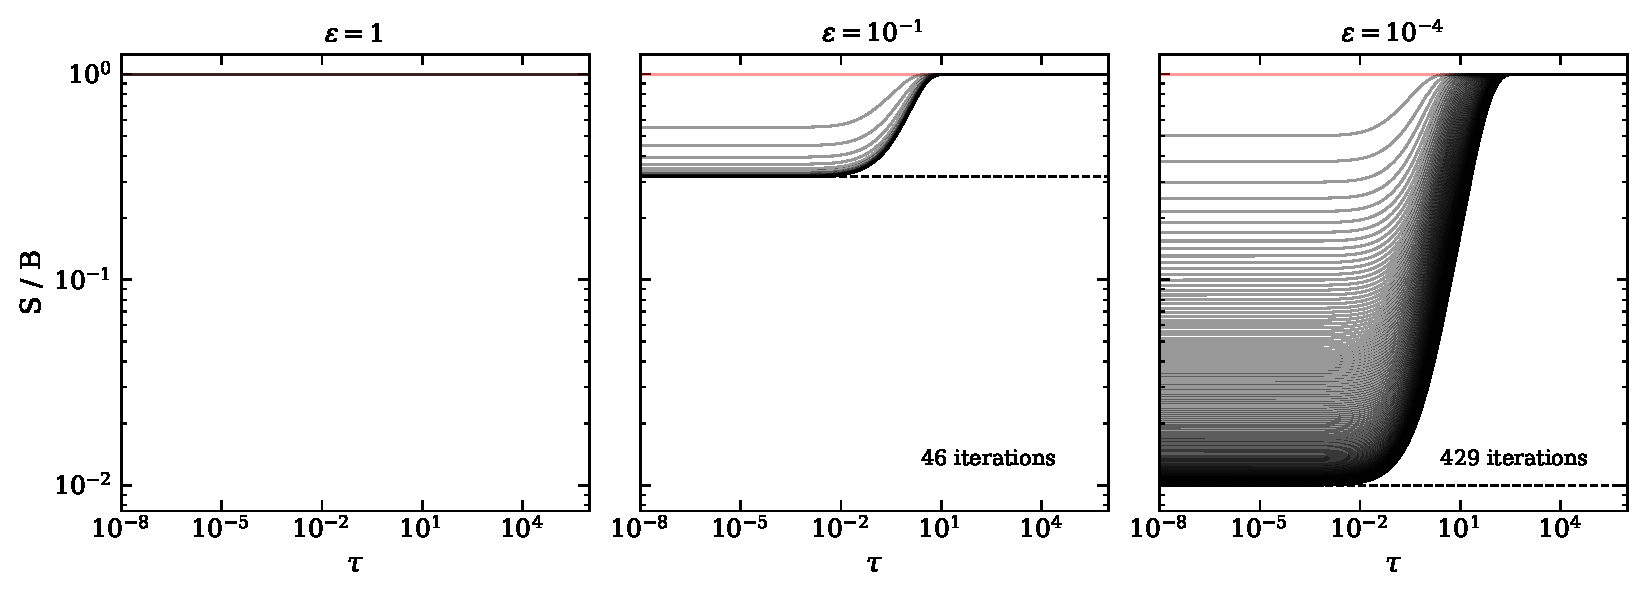
\includegraphics[width=0.99\textwidth]{eps_convergence.pdf}
 \caption{Convergence plots for different values of $\epsilon$. As $\epsilon$ approaches 0, more iterations are needed to achieve convergence at the surface.}
   \label{fig:2}
\end{figure}

As a test of the final product of the formal solution, we plot a spectrum generated from our model to ensure we obtain an expected blackbody curve. \autoref{fig:3} shows the emergent flux of our model post-convergence at a set of wavelength points between 3000 and 7000 \text{\AA}. It is clear that we indeed achieve the expected result with no unexpected variation as a function of wavelength.

\begin{figure}[ht]
 \centering
 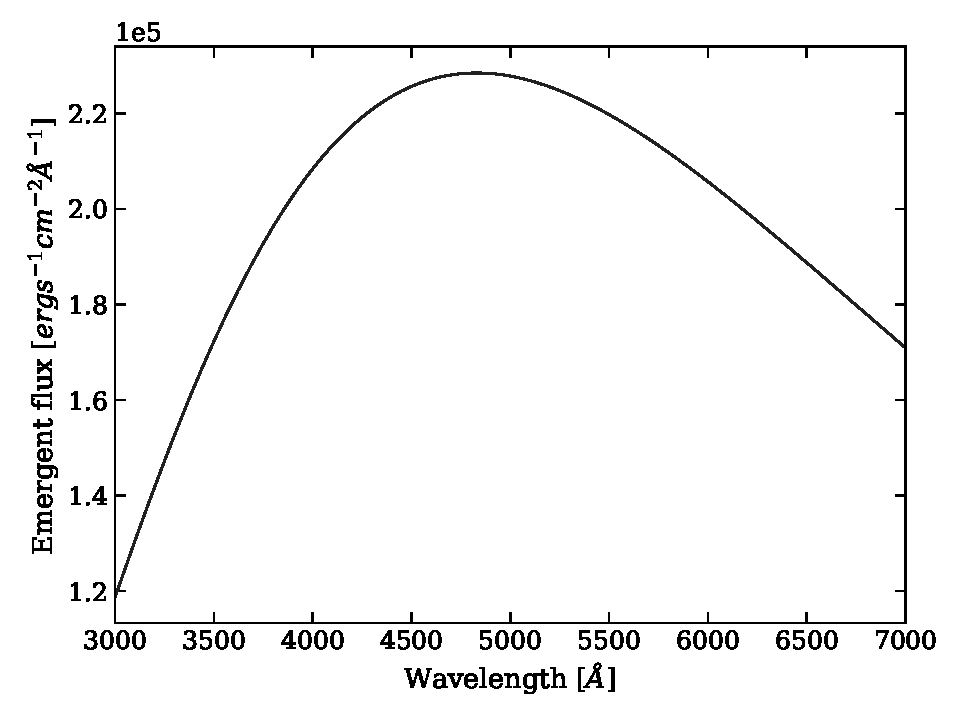
\includegraphics[width=0.75\textwidth]{spectrum.pdf}
 \caption{Output spectrum using the default parameters. The line feature at 6564 \text{\AA } appears, however the shape is incorrect.}
  \label{fig:3}
\end{figure}

Since $J$ is the direction-averaged intensity, comparing our $J$ to an analytic value is important as it directly relates to flux from the atmosphere. In \autoref{fig:4}, we show the percent difference between our calculated $J$ and the $J$ calculated by using the analytic approximation assuming $B$ is linear in $\tau$,
\begin{align}
J(\tau) = a + b\tau + \frac{(b - \sqrt{3}a)e^{-\sqrt{3\epsilon}}}{(\sqrt{3}+\sqrt{3\epsilon})},
\label{eq:24}
\end{align}
however with $b = 0$ because we assume an isothermal atmosphere. The largest difference between our calculated $J$ and the analytic solution occurs from $10^{-2} < \tau < 1$. This is expected, as this region around $\tau \approx 2/3$ is typically characteristic of the emergent flux of the atmosphere. Elsewhere, there is little divergence between results. We vary $\epsilon$ as well for this test, but we do not obtain significant changes as $\epsilon$ varies.

\begin{figure}[ht]
 \centering
 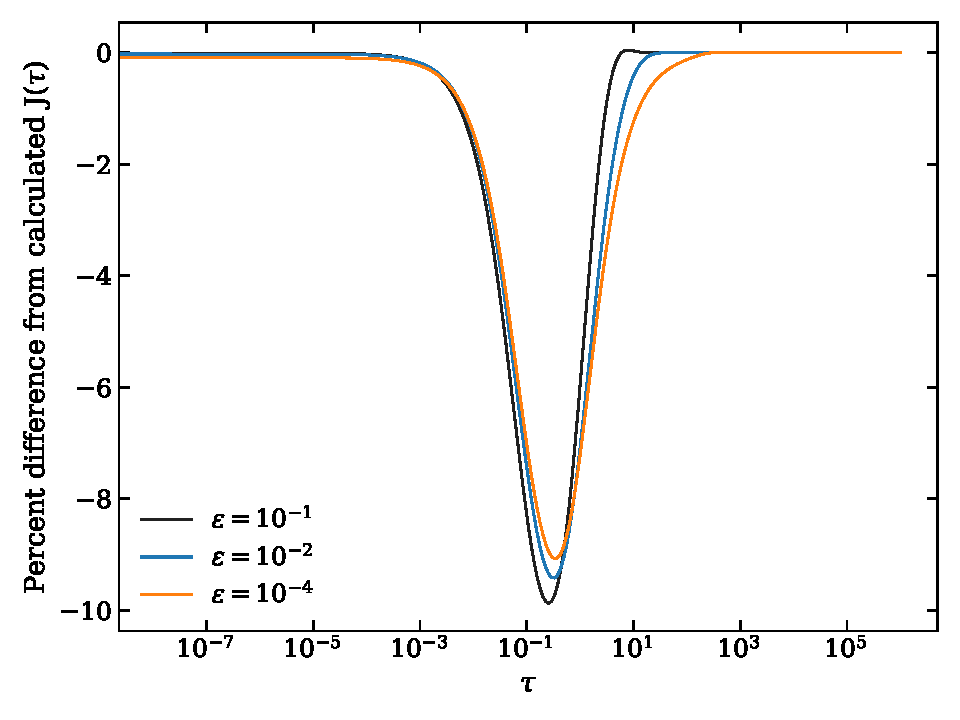
\includegraphics[width=0.75\textwidth]{J_comparison.pdf}
 \caption{Comparison of our J to the analytic solution. The greatest differences occur around $\tau = 2/3$, where we expect the greatest impact in the emergent flux from the atmosphere. Varying $\epsilon$ does not impact J to a significant degree.}
 \label{fig:4}
\end{figure}


\subsection{Effects of Gauss-Legendre Quadrature}
\label{sec:quad}


We also investigate the effect of choosing fewer $\mu$ values when integrating using Gauss-Legendre quadrature. Ideally one uses as many points as possible for higher degrees of accuracy in the integration to get the formal solution, however this of course increases computation time. In \autoref{fig:5} we display the percent difference in $S_2$, $S_4$, and $S_8$, where $S_n$ is the $S$ calculated for $n$-point quadrature, compared to the 32-point result we typically use, $S_{32}$. The figure shows that if we use fewer points, our calculated source function deviates significantly in the same $\tau \approx 2/3$ regime.

To test the resulting time it takes to generate a typical model for these different cases, we simply calculate a spectrum similarly to that in \autoref{sec:ali} for ~170 wavelength points, which includes the same check for convergence at each step that was described also in \autoref{sec:ali}. On average, for the 2-, 4-, 8-, and 32-point methods, these spectra were able to be generated in 3.629, 3.484, 3.583, and 4.238 seconds, respectively. This means that calculations using 2, 4, and 8 points are faster than 32 points by 14\%, 18\%, and 15\%, respectively, but at worst only 9\%, 4\%, and 2\% less accurate. With the same number of iterations, one would expect computation time to increase linearly with the number of points used in integration. With that in mind, the results imply that, when using fewer points, it takes longer to reach the convergence criterion for the same number of iterations when using fewer points.

Although a few seconds for a simple calculation is not much, it is interesting to note this effect for doing radiative transfer on a larger scale, and the possible results that may propagate from the convergence step in the big picture that ALI addresses.

\begin{figure}[ht]
 \centering
 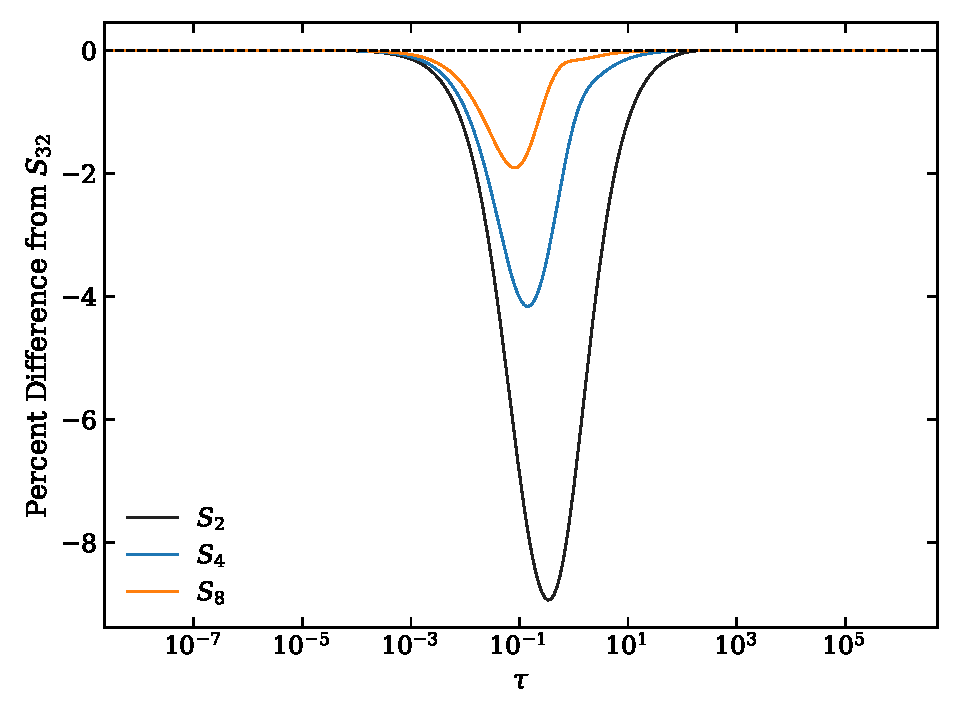
\includegraphics[width=0.75\textwidth]{quadrature.pdf}
 \caption{Deviations from 32-point Gaussian quadrature as a function of $\tau$. Similarly to Figure 4, the greatest difference occurs from $0.1 < \tau < 1$. }
 \label{fig:5}
\end{figure}


\subsection{Effects of Ng Acceleration}


Finally, we investigate the effects of Ng acceleration described in \autoref{sec:ng} on the speed of convergence. The left panel in \autoref{fig:6} shows the number of iterations required to reach convergence at the surface for $\epsilon = 10^{-4}$ for normal lambda iteration (LI), ALI, and ALI with Ng acceleration implemented. As expected, ALI converges much faster than LI, with Ng acceleration further reducing the required number of iterations. The right panel shows the same result in essence, however this is specifically showing the maximum value used to check convergence $\Delta J / \bar{J}$ across all $\tau$. In other words, the dashed line in this right panel at $10^{-8}$ is our definition of convergence. This gives us an idea of how significantly $J$ itself changes, and it shows again the same sentiment, that Ng acceleration converges in fewer iterations compared to both LI and ALI. LI in particular does not perform well to minimize this quantity, and it would require a drastically higher number iterations to achieve the same result.

\begin{figure}[ht]
 \centering
 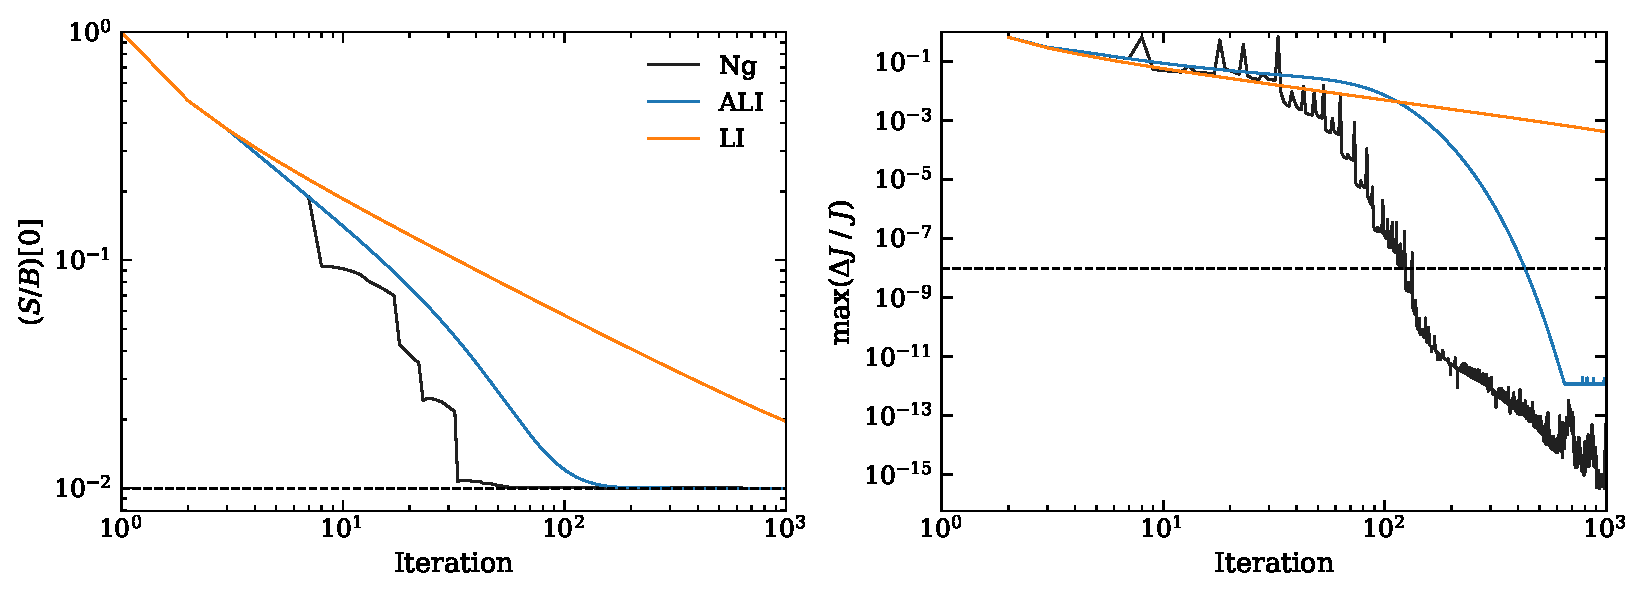
\includegraphics[width=0.99\textwidth]{iterations.pdf}
 \caption{Left: The number of iterations required for S/B to converge at the surface for each method used in our code. Lambda iteration takes significantly longer than ALI as expected. Ng acceleration improves the required number of iterations even further. The jagged pattern is a result of how the algorithm is designed. Right: Variations in J as a function of iteration. Ng acceleration minimizes the change in J faster than ALI, though this does not take effect until about 40 iterations, and then levels off before dropping again at 700 iterations.}
  \label{fig:6}
\end{figure}

In \autoref{fig:7}, we plot the same convergence test as in \autoref{fig:1}, however now implementing Ng acceleration. We see that there are large gaps in $S / B$ every time the algorithm described in \autoref{sec:ng} makes a new estimate of $S$. Clearly this method works to reduce the number of iterations required to fully converge $J$.

\begin{figure}[ht]
 \centering
 \includegraphics[width=0.75\textwidth]{doc/figs/S_B_convergence.pdf}
 \caption{The same convergence plot as Figure 1 but with Ng acceleration implemented. The number of iterations required for convergence decreases significantly.}
  \label{fig:7}
\end{figure}

Finally, we perform a similar test as in \autoref{sec:quad}, however now to see how quickly $J$ converges and a spectrum may be generated using the different iteration methods. On average, ALI takes 4.222 seconds, and ALI with Ng acceleration takes 1.695 seconds. LI was not included as the number of iterations it would take to converge with $\epsilon = 10^{-4}$ is significantly longer than ALI and frankly is not worth the time spent to compute it.


\section{Conclusion}


In this project, we implemented accelerated lambda iteration in order to solve the radiative transfer equation and the NLTE scattering problem. We have tested the results thoroughly for an isothermal, grey atmosphere, which have all had positive results that show our method to be successful in capturing the expected behavior for a solution to the radiative transfer problem. We also show that ALI is able to converge much faster than normal lambda iteration, which is useful for computational efficiency. Finally, we make use of Ng acceleration, and show that such a simple implementation is able to solve such a complicated problem using drastically less time and resources.

Our implementation of this method is available at \href{https://github.com/anthonyburrow/Rad1D}{github.com/anthonyburrow/Rad1D} wherein all parameters available for any user to test this method are shown and described.


\clearpage
\bibliography{FinalProjectReport}

\end{document}
